\documentclass[10pt, aspectratio=169]{beamer}
\usetheme{Madrid}

% Professional Color Palette (Navy / Slate Gray / Muted Gold)
\definecolor{NavyBlueCustom}{RGB}{20, 35, 60}
\definecolor{SlateGrayCustom}{RGB}{80, 95, 110}
\definecolor{GoldCustom}{RGB}{190, 140, 40}
\definecolor{LightBgCustom}{RGB}{248, 249, 250}

\setbeamercolor{palette primary}{bg=NavyBlueCustom,fg=white}
\setbeamercolor{palette secondary}{bg=SlateGrayCustom,fg=white}
\setbeamercolor{palette tertiary}{bg=NavyBlueCustom,fg=white}
\setbeamercolor{titlelike}{bg=NavyBlueCustom,fg=white}
\setbeamercolor{frametitle}{bg=NavyBlueCustom,fg=white}
\setbeamercolor{structure}{fg=NavyBlueCustom}
\setbeamercolor{block title}{bg=NavyBlueCustom,fg=white}
\setbeamercolor{block body}{bg=LightBgCustom,fg=black}

% Bullet style: circles instead of arrows
\setbeamertemplate{itemize item}[circle]
\setbeamertemplate{itemize subitem}[circle]
\setbeamertemplate{itemize subsubitem}[circle]
\setbeamercolor{itemize item}{fg=GoldCustom}
\setbeamercolor{itemize subitem}{fg=SlateGrayCustom}

\setbeamertemplate{navigation symbols}{}

\usepackage[utf8]{inputenc}
\usepackage{amsmath}
\usepackage{amssymb}
\usepackage{listings}
\usepackage{tikz}
\usetikzlibrary{positioning, arrows.meta, shapes}

\lstset{
  basicstyle=\ttfamily\small,
  breaklines=true,
  frame=single,
  backgroundcolor=\color{gray!10}
}

\title{Week 1: Introduction to Computing Systems \& Binary Foundations}
\subtitle{Abstraction Layers, Binary, Two's Complement, Hex, and the Iron Law}
\author{J. Burns}
\institute{CSCI 6461 --- Computer Systems Architecture}
\date{\today}

\begin{document}

% ============================================================
\begin{frame}
\titlepage
\end{frame}

% ============================================================
\section{Framing \& Motivation}

\begin{frame}{Why Study Computer Architecture?}
\begin{itemize}
    \item Every line of software eventually becomes voltages on wires
    \item Performance, energy efficiency, and correctness are all bounded by hardware
    \item Understanding the stack lets you reason about \emph{why} code is slow, not just \emph{that} it is slow
    \item Architecture knowledge is essential for: compiler writers, OS designers, systems programmers, ML/HPC engineers
    \item This week builds the vocabulary, number systems, and performance model used for the rest of the course
\end{itemize}
\end{frame}

\begin{frame}{The Great Abstraction Stack}
\begin{center}
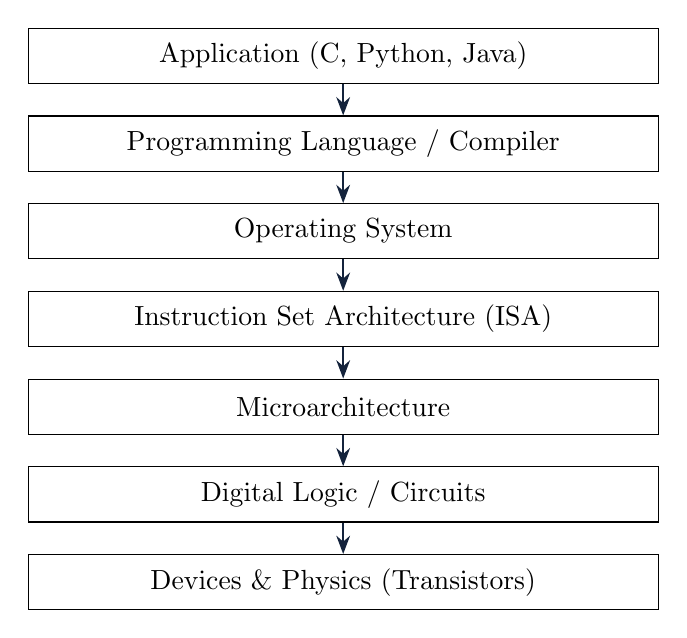
\begin{tikzpicture}[node distance=0.4cm, every node/.style={rectangle, draw, minimum width=8cm, minimum height=0.7cm}]
\node (app) {Application (C, Python, Java)};
\node (lang) [below=of app] {Programming Language / Compiler};
\node (os) [below=of lang] {Operating System};
\node (isa) [below=of os] {Instruction Set Architecture (ISA)};
\node (uarch) [below=of isa] {Microarchitecture};
\node (circ) [below=of uarch] {Digital Logic / Circuits};
\node (dev) [below=of circ] {Devices \& Physics (Transistors)};
\draw[-Stealth, thick, NavyBlueCustom] (app) -- (lang);
\draw[-Stealth, thick, NavyBlueCustom] (lang) -- (os);
\draw[-Stealth, thick, NavyBlueCustom] (os) -- (isa);
\draw[-Stealth, thick, NavyBlueCustom] (isa) -- (uarch);
\draw[-Stealth, thick, NavyBlueCustom] (uarch) -- (circ);
\draw[-Stealth, thick, NavyBlueCustom] (circ) -- (dev);
\end{tikzpicture}
\end{center}
\end{frame}

\begin{frame}{Learning Objectives}
By the end of Week 1, students should be able to:
\begin{itemize}
    \item Trace a program's journey from C source to gate-level control signals
    \item Convert fluently between binary, decimal, and hexadecimal
    \item Represent and manipulate signed integers using two's complement
    \item Detect overflow and correctly perform sign extension
    \item Apply the Iron Law of performance to compare machine designs
\end{itemize}
\end{frame}

% ============================================================
\section{Abstraction Layers in Practice}

\begin{frame}{From C to Machine: The Compilation Pipeline}
\begin{center}
\texttt{source.c} $\rightarrow$ \textbf{Preprocessor} $\rightarrow$ \textbf{Compiler} $\rightarrow$
\texttt{.s} (assembly) $\rightarrow$ \textbf{Assembler} $\rightarrow$ \texttt{.o} (object) $\rightarrow$
\textbf{Linker} $\rightarrow$ \texttt{a.out} $\rightarrow$ \textbf{Loader} $\rightarrow$ execution
\end{center}
\vspace{0.3cm}
\begin{itemize}
    \item Preprocessor: macro expansion, \texttt{\#include} resolution
    \item Compiler: translates high-level constructs to assembly, performs optimization
    \item Assembler: translates mnemonics to machine encodings
    \item Linker: resolves symbols across object files and libraries
    \item Loader: places the executable image into memory and starts execution
\end{itemize}
\end{frame}

\begin{frame}[fragile]{A Simple C Function}
We will trace this function through every layer of the stack:
\begin{lstlisting}
int add(int a, int b) {
    return a + b;
}
\end{lstlisting}
\begin{itemize}
    \item Simple enough to see every transformation clearly
    \item Involves register usage, arithmetic, and function return conventions
    \item We'll revisit this same example at each layer
\end{itemize}
\end{frame}

\begin{frame}{RISC Design Philosophy}
ARM64 (and RISC-V) embody the classic RISC principles:
\begin{itemize}
    \item \textbf{Fixed-width instructions} (32 bits, always) -- simplifies fetch and decode, enables easy pipelining
    \item \textbf{Load/store architecture} -- only \texttt{LDR}/\texttt{STR} touch memory; arithmetic instructions operate strictly on registers
    \item \textbf{Large, uniform register file} -- 31 general-purpose 64-bit registers (\texttt{x0--x30}) reduce memory traffic
    \item \textbf{Simple addressing modes} -- fewer, more regular formats compared to CISC (e.g., x86)
    \item Consequence: instructions are individually simpler $\Rightarrow$ CPI (Cycles Per Instruction -- covered in detail later in the Iron Law section) tends toward 1, but instruction \emph{count} for a given task can be higher than a CISC ISA
\end{itemize}
\end{frame}

\begin{frame}[fragile]{C $\rightarrow$ Assembly (Compiler's Job)}
\begin{lstlisting}
add:
    add  w0, w0, w1    ; w0 = a + b  (args in w0, w1)
    ret                ; return value in w0, return addr in x30
\end{lstlisting}
\begin{itemize}
    \item AArch64 (ARM64) calling convention: first arguments in \texttt{w0/x0}, \texttt{w1/x1}, \dots; return value in \texttt{w0/x0}
    \item No explicit \texttt{mov} needed -- RISC compilers lean on a large uniform register file rather than shuffling values
    \item \texttt{ret} implicitly branches to the link register \texttt{x30} -- no explicit operand required in the common case
\end{itemize}
\end{frame}

\begin{frame}{Assembly $\rightarrow$ Machine Code (Assembler's Job)}
\begin{center}
\begin{tabular}{l l}
\textbf{Assembly} & \textbf{Machine Code (hex)} \\
\hline
\texttt{add w0, w0, w1} & \texttt{0x0B010000} \\
\texttt{ret} & \texttt{0xD65F03C0} \\
\end{tabular}
\end{center}
\begin{itemize}
    \item Every ARM64 instruction is exactly 32 bits -- opcode, registers, and immediates sit in fixed bit fields
    \item Fixed width means the decoder never has to first figure out ``how long is this instruction?'' (unlike variable-length CISC encodings)
    \item Assembler resolves labels into PC-relative offsets encoded directly in the instruction word
\end{itemize}
\end{frame}

\begin{frame}{Machine Code $\rightarrow$ Gates (Hardware's Job)}
\begin{itemize}
    \item CPU fetches a fixed 32-bit instruction word from memory every cycle
    \item Control unit decodes fixed bit fields (opcode, \texttt{Rn}, \texttt{Rm}, \texttt{Rd}, immediate) into control signals
    \item Control signals drive muxes, ALU operation select lines, register file read/write enables
    \item Fixed-width, regular encoding is precisely what makes single-cycle decode -- and later, pipelined decode -- tractable
    \item This is the boundary where software becomes physics
\end{itemize}
\end{frame}

\begin{frame}{Why Abstraction Works: Isolation of Concerns}
\begin{itemize}
    \item Each layer exposes an interface and hides implementation details from the layer above
    \item A compiler writer doesn't need to know transistor physics
    \item A circuit designer doesn't need to know C syntax
    \item Enables independent innovation at each layer (e.g., new microarchitectures behind the same ISA)
    \item Cost: some inefficiency and information loss at each boundary
\end{itemize}
\end{frame}

\begin{frame}{Where Abstraction Leaks}
\begin{itemize}
    \item \textbf{Cache effects}: identical algorithms, wildly different runtimes depending on memory access pattern
    \item \textbf{Undefined behavior}: C's abstraction assumes well-defined semantics that hardware doesn't always guarantee
    \item \textbf{Timing side-channels}: Spectre/Meltdown show microarchitectural state leaking through the ISA boundary
    \item \textbf{Numerical representation}: floating-point rounding is invisible until it isn't
    \item Architecture knowledge lets you reason \emph{across} layers when abstraction breaks down
\end{itemize}
\end{frame}

% ============================================================
\section{Unsigned Binary}

\begin{frame}{Why Binary? Physical \& Engineering Motivation}
\begin{itemize}
    \item Transistors are most reliably operated as two-state switches (on/off)
    \item Two voltage levels give large noise margins compared to multi-level encoding
    \item Binary logic maps directly onto Boolean algebra $\Rightarrow$ clean mathematical foundation
    \item Alternative bases (e.g., ternary computing) exist but lack the same manufacturing maturity
\end{itemize}
\end{frame}

\begin{frame}{Positional Number Systems Review}
\begin{itemize}
    \item A number in base $b$ with digits $d_{n-1} \ldots d_1 d_0$ represents:
    \[
    \sum_{i=0}^{n-1} d_i \cdot b^i
    \]
    \item Decimal (base 10): digits $0$--$9$
    \item Binary (base 2): digits $0$--$1$
    \item Example: $(503)_{10} = 5\times10^2 + 0\times10^1 + 3\times10^0$
\end{itemize}
\end{frame}

\begin{frame}{Unsigned Binary Representation}
\begin{itemize}
    \item $n$-bit unsigned number: $\sum_{i=0}^{n-1} b_i \cdot 2^i$, where $b_i \in \{0,1\}$
    \item Range: $0$ to $2^n - 1$
    \item Example (8 bits): $0000\,0000$ to $1111\,1111$ = $0$ to $255$
    \item Most significant bit (MSB) carries weight $2^{n-1}$
\end{itemize}
\end{frame}

\begin{frame}{Binary $\leftrightarrow$ Decimal Conversion}
\textbf{Binary to Decimal:} sum the weights of set bits
\[
1011_2 = 1\times8 + 0\times4 + 1\times2 + 1\times1 = 11_{10}
\]
\textbf{Decimal to Binary:} repeated division by 2 (record remainders)
\[
13 \div 2 = 6\ r1,\ 6 \div 2 = 3\ r0,\ 3 \div 2 = 1\ r1,\ 1 \div 2 = 0\ r1 \Rightarrow 1101_2
\]
\end{frame}

\begin{frame}{Binary Addition}
\begin{itemize}
    \item Same rules as decimal addition, base 2 carry rules:
    \item $0+0=0$, \quad $0+1=1$, \quad $1+1=10$ (write 0, carry 1), \quad $1+1+1=11$
\end{itemize}
\[
\begin{array}{r}
 0111 \\
+0101 \\
\hline
 1100
\end{array}
\]
\begin{itemize}
    \item Carry chain ripples left-to-right -- this is exactly how a ripple-carry adder circuit works
    \item Overflow (for unsigned) occurs when there's a carry out of the MSB
\end{itemize}
\end{frame}

\begin{frame}{Bit Widths and Range Limits}
\begin{center}
\begin{tabular}{l l l}
\textbf{Width} & \textbf{Unsigned Range} & \textbf{Common Use} \\
\hline
8-bit  & 0 -- 255 & byte, char \\
16-bit & 0 -- 65{,}535 & short \\
32-bit & 0 -- $\sim$4.29 billion & int, \texttt{w}-registers (ARM64) \\
64-bit & 0 -- $\sim$1.8$\times10^{19}$ & long, \texttt{x}-registers, pointers \\
\end{tabular}
\end{center}
\begin{itemize}
    \item Choice of width is a real design/cost tradeoff: storage, bus width, register size
    \item Overflow silently wraps around in unsigned arithmetic -- a common bug source
\end{itemize}
\end{frame}

% ============================================================
\section{Two's Complement}

\begin{frame}{The Problem with Naive Signed Representations}
\textbf{Sign-magnitude:} reserve MSB as sign bit, remaining bits as magnitude
\begin{itemize}
    \item Example (4-bit): $0101 = +5$, $1101 = -5$
    \item \textbf{Problem:} two representations of zero ($0000$ and $1000$); addition needs separate sign-handling logic
    \item \textbf{One's complement} (brief note): negative = bitwise NOT of positive; still has dual-zero problem ($0000$/$1111$) and needs ``end-around carry'' correction
    \item Used historically (CDC, some UNIVAC systems); both abandoned in favor of two's complement
    \item Motivates a representation where addition ``just works'' with a single circuit
\end{itemize}
\end{frame}

\begin{frame}{Two's Complement Definition}
\begin{itemize}
    \item Standard signed integer representation in virtually all modern architectures, including ARM64 and RISC-V
    \item For $n$ bits, value is:
    \[
    -b_{n-1}\cdot 2^{n-1} + \sum_{i=0}^{n-2} b_i \cdot 2^i
    \]
    \item Intuition: the MSB has \emph{negative} weight
    \item Range for $n$ bits: $-2^{n-1}$ to $2^{n-1}-1$ (asymmetric!)
    \item Exactly one representation of zero
\end{itemize}
\end{frame}

\begin{frame}{Two's Complement: Computing the Negative}
\textbf{Algorithm:} invert all bits, then add 1
\[
+5 = 0101 \xrightarrow{\text{invert}} 1010 \xrightarrow{+1} 1011 = -5
\]
\begin{itemize}
    \item Equivalent shortcut: copy bits up to and including the first 1 (from the right), invert the rest
    \item Negating twice returns the original value (except for the most-negative edge case)
    \item Circuit implication: negation reuses the same adder as addition (add inverted operand + 1) -- no separate ``negate'' circuit needed
\end{itemize}
\end{frame}

\begin{frame}{Two's Complement Addition/Subtraction}
\begin{itemize}
    \item Addition: identical bit-level procedure as unsigned addition -- \emph{same hardware}
    \item Subtraction: $A - B = A + (\text{two's complement of } B)$
    \item This uniformity is precisely \emph{why} two's complement won out over sign-magnitude / one's complement
\end{itemize}
\[
\begin{array}{r}
 0011\ (+3) \\
+1110\ (-2) \\
\hline
 0001\ (+1)\ \text{(carry out discarded)}
\end{array}
\]
\end{frame}

\begin{frame}{Overflow Detection in Two's Complement}
\begin{itemize}
    \item Unsigned overflow $\ne$ signed overflow -- must check separately
    \item \textbf{Rule:} signed overflow occurs when two operands of the \emph{same sign} produce a result of the \emph{opposite sign}
    \item \textbf{Circuit rule:} overflow = XOR of carry-into-MSB and carry-out-of-MSB
    \item Example: $0111\ (+7) + 0001\ (+1) = 1000\ (-8)$ -- overflow! (positive + positive = negative)
    \item ARM64 makes this explicit in hardware: the \texttt{NZCV} condition flags register sets \texttt{N} (negative), \texttt{Z} (zero), \texttt{C} (carry/unsigned overflow), \texttt{V} (signed overflow) after flag-setting instructions like \texttt{ADDS}/\texttt{SUBS} or \texttt{CMP}
\end{itemize}
\end{frame}

\begin{frame}{Sign Extension}
\begin{itemize}
    \item Widening a signed value to more bits must preserve its numeric value
    \item \textbf{Rule:} replicate the sign bit (MSB) into all new upper bits
    \item Example: 4-bit $-5 = 1011 \rightarrow$ 8-bit $= 1111\,1011$ (still $-5$)
    \item Contrast with unsigned \emph{zero extension}: pad with 0s instead
    \item ARM64 provides dedicated instructions: \texttt{SXTW}, \texttt{SXTB}/\texttt{SXTH} for sign extension; \texttt{UXTW} etc. for zero extension. RISC-V analog: \texttt{sext.w}
\end{itemize}
\end{frame}

% ============================================================
\section{Hexadecimal \& Bit Manipulation}

\begin{frame}{Hexadecimal Representation}
\begin{itemize}
    \item Base 16, digits $0$--$9$ then $A$--$F$ (10--15)
    \item Compact, human-friendly shorthand for binary
    \item One hex digit = exactly 4 bits (one ``nibble'')
    \item Written with prefix \texttt{0x} in most programming languages and in ARM64/RISC-V assembly
\end{itemize}
\end{frame}

\begin{frame}{Binary $\leftrightarrow$ Hex Conversion}
\textbf{Technique:} group binary into nibbles (groups of 4) from the right
\[
1011\,1100\,0110_2 \;\rightarrow\; \underbrace{1011}_{B}\ \underbrace{1100}_{C}\ \underbrace{0110}_{6} \;=\; \texttt{0xBC6}
\]
\begin{itemize}
    \item Reverse direction: expand each hex digit into its 4-bit binary equivalent
    \item Much faster than converting through decimal
\end{itemize}
\end{frame}

\begin{frame}{Hex in Practice}
\begin{itemize}
    \item Memory addresses: \texttt{0x0000\,FFFF\,7FFE\,A3C0}
    \item Register/debugger dumps -- compact display of 32-bit (\texttt{w}) / 64-bit (\texttt{x}) register values
    \item Color codes as a familiar analogy: \texttt{\#FF5733} is really 3 bytes in hex
    \item Instruction encodings, hash digests, and binary file inspection (\texttt{hexdump}, \texttt{xxd})
\end{itemize}
\end{frame}

\begin{frame}{Bitwise Operations}
\begin{center}
\begin{tabular}{l l l}
\textbf{Op} & \textbf{C Symbol} & \textbf{ARM64 Mnemonic} \\
\hline
AND & \texttt{\&} & \texttt{AND} \\
OR  & \texttt{|} & \texttt{ORR} \\
XOR & \texttt{\^{}} & \texttt{EOR} \\
NOT & \texttt{\~{}} & \texttt{MVN} \\
Shift left/right & \texttt{<<}\ \texttt{>>} & \texttt{LSL} / \texttt{LSR} (logical), \texttt{ASR} (arithmetic) \\
\end{tabular}
\end{center}
\begin{itemize}
    \item Each maps to a dedicated, single-cycle ALU function unit in hardware
    \item RISC ISAs expose logical vs.\ arithmetic shift as \emph{distinct} instructions -- the difference matters for signed two's complement values
\end{itemize}
\end{frame}

\begin{frame}{Practical Encoding Example}
\begin{itemize}
    \item Character \texttt{'A'} $\rightarrow$ ASCII decimal $65$ $\rightarrow$ binary $0100\,0001$ $\rightarrow$ hex \texttt{0x41}
    \item String \texttt{"Hi"} stored as consecutive bytes: \texttt{0x48 0x69}
    \item Demonstrates all three representations (binary/decimal/hex) describing the \emph{same} underlying bit pattern
    \item Reinforces: representation is a lens, not a property of the data itself
\end{itemize}
\end{frame}

% ============================================================
\section{Basic CPU Performance Metrics: The Iron Law}

\begin{frame}{What Do We Mean by ``Performance''?}
\begin{itemize}
    \item \textbf{Latency}: time to complete a single task (seconds)
    \item \textbf{Throughput}: tasks completed per unit time (tasks/second)
    \item Optimizing one does not always optimize the other (e.g., pipelining improves throughput, may not reduce single-instruction latency)
    \item Architecture decisions are always latency/throughput/energy tradeoffs
\end{itemize}
\end{frame}

\begin{frame}{The Iron Law of Performance}
\[
\text{CPU Time} = \text{Instruction Count} \times \text{CPI} \times \text{Clock Cycle Time}
\]
\begin{itemize}
    \item \textbf{Instruction Count (IC):} dynamic instructions executed -- depends on the program, compiler, and ISA (RISC vs.\ CISC)
    \item \textbf{CPI:} cycles per instruction -- depends on microarchitecture
    \item \textbf{Clock Cycle Time:} $1/\text{clock rate}$ -- depends on circuit design \& fabrication technology
    \item Called the \emph{Iron Law} because every architectural decision you make moves exactly one of these three knobs -- and often trades off against another
\end{itemize}
\end{frame}

\begin{frame}{Clock Rate, Cycle Time, and Frequency}
\begin{itemize}
    \item Clock rate $f$ measured in Hz; cycle time $T = 1/f$
    \item Example: $3\ \text{GHz} \Rightarrow T \approx 0.33\ \text{ns}$
    \item Historical trend: clock rates scaled aggressively through the early 2000s (Dennard scaling), then plateaued due to power/heat limits
    \item Since then, performance gains increasingly come from parallelism (multicore, wider pipelines, SIMD) rather than raw frequency -- the third term of the Iron Law has stagnated, so architects push harder on IC and CPI
\end{itemize}
\end{frame}

\begin{frame}{CPI and Instruction Mix}
\begin{itemize}
    \item Different instruction classes have different costs (e.g., loads vs.\ ALU ops vs.\ branches)
    \item Overall CPI is a weighted average:
    \[
    \text{CPI} = \sum_{i} \left( \text{Freq}_i \times \text{CPI}_i \right)
    \]
    \item In a load/store RISC ISA, ALU ops are register-only and cheap; only \texttt{LDR}/\texttt{STR} touch memory and carry the largest cost
    \item Example (ARM64-like mix): 50\% ALU (CPI=1), 30\% load/store (CPI=4), 20\% branch (CPI=2)
    \item $\text{CPI} = 0.5(1) + 0.3(4) + 0.2(2) = 2.1$
    \item RISC bet: simple instructions push CPI toward 1, even if IC is somewhat higher than a CISC ISA doing the same task
\end{itemize}
\end{frame}

\begin{frame}{Worked Iron Law Problem}
Two machines run the same program (100M instructions):
\begin{itemize}
    \item \textbf{Machine A:} 2 GHz clock, CPI = 1.5
    \item \textbf{Machine B:} 3 GHz clock, CPI = 2.5
\end{itemize}
\[
T_A = \frac{100\times10^6 \times 1.5}{2\times10^9} = 75\ \text{ms}
\qquad
T_B = \frac{100\times10^6 \times 2.5}{3\times10^9} \approx 83.3\ \text{ms}
\]
\begin{itemize}
    \item Machine A is faster despite the lower clock rate -- higher frequency alone doesn't guarantee better performance
    \item This is the Iron Law in action: all three terms must be considered together, never just one in isolation
\end{itemize}
\end{frame}

% ============================================================
\section{Synthesis}

\begin{frame}{Recap \& Bridge to Week 2}
\begin{itemize}
    \item The abstraction stack lets software and hardware evolve independently -- but leaks matter at the architecture level
    \item Two's complement unifies signed/unsigned addition into one circuit -- a recurring design theme: \emph{reuse hardware across cases}
    \item Hex is binary's human-readable shorthand; bitwise ops map directly to ARM64 ALU instructions
    \item The Iron Law (IC $\times$ CPI $\times$ Cycle Time) is the lens for every optimization we'll study this term
    \item \textbf{Week 2:} Instruction Set Architecture design -- how instructions are chosen, encoded, and how ISA choices shape IC and CPI
\end{itemize}
\end{frame}

\end{document}